\documentclass[a4paper]{article} % a4paper option recommended
\usepackage[english]{babel}
\usepackage{uureport}
\usepackage{cite}
\usepackage{hyperref}
\usepackage{pgfplots}
\usepackage{float}
\usepackage{listings}
\usepackage{graphicx}
\usepackage{amsmath}
\bibliographystyle{alpha}


\title{Diplomacy}
\type{Report}
\course{Games \& Agents}

\author{A. Berland, B. Reigersberg, E. Koens, \\J. de Groot, K. van Katwijk, T. de Goeij}

\begin{document}
\maketitle
\tableofcontents
\newpage

\section{Introduction}
Diplomacy is an online multiplayer game based on the board game invented in 1954 by Allan B. Calhamer. The online version of the game has 137966 subscribed players at time of writing. However, it can be played by bots as well. A few bots have already been implemented and a number of tools have been created to make implementing bots easier (such as servers that people can run at home and a syntax named the 'Diplomacy AI Development Environment Message Syntax' that allows bots to communicate with one another). So far the best bot on the market is a bot named Albert, created by Jason van Hal. All these bots lack one common property, which is the ability to assess the other players. 
\\We created a bot named DodoAI that will attempt to comprehend, judge, predict and learn from the actions and behaviours of the competing players. Our bot can deduce the best possible moves which are based on his own ideas and observations, he will also concern his current belief on the other player or bot. We made quite some progress and we will elaborate on our development of this bot in this paper.

\subsection{Diplomacy}
The online Diplomacy game is based on the map of 1901 Europe, though it can also be played on other (non-standard) maps. The map consists of three different kinds of provinces. These types are land provinces, coastal provinces and sea provinces. Land provinces and coastal provinces may contain a so-called Supply Center.
\\The goal of the game is to be the first of seven players to hold more than half of the Supply Centers that are available on the map (the standard map has 34 Supply Centers). Supply Centers can be divided in two types: Home Supply Centers and other Supply Centers (there is difference between these to types in the game itself when it comes to scoring but we considered the difference for the sake of the weight \& gains system which will be explained later). All Supply Centers sustain the military units, however only Home Supply Centers can build new units. In order to build new units a player has to own more Supply Centers than units this is done in the Build phase (Winter).
\\There are five phases in Diplomacy, as stated earlier there is the Build phase, which is called Winter in game. There are two Order phases (Summer and Fall) in which the player may decide where to move his available units. After each Order phase there is a Retreat phase (Spring and Autumn). In the Retreat phase any units that were attacked and failed to defend themselves are forced to retreat. If there is no possible place to retreat to the unit needs to be disbanded (removed from the game).
\\The players control two different types of units. On one side there is the Army unit type which moves on coastal and land provinces. The other unit type is the Fleet, this unit can move through coastal provinces and trough oceans.
\\The units have five types of moves. The first move is the HOLD move. With this move the unit stays on its current province in order to defend it against invading units.
The second type of action is the MOVE action, with it the unit moves from one province into an adjacent province. When a unit tries to move into a province that is already occupied by another player then the unit will attack the target province. The attack will succeed if the attacking unit's power exceeds the defending unit's power. The units are all considered to be equally powerful, so in order to successfully invade or defend a province a unit may receive support from another unit.
There are two types of support moves, the SUPPORT HOLD, this is a support for the defending HOLD move. The SUPPORT HOLD gives the defending army an additional unit to defend with. And then there is the SUPPORT MOVE, which is basically the same but for attacking. The last move is the CONVOY move, for this move a player needs both a Fleet and an adjacent Army. The Fleet needs to be in an ocean province. The Army may then move across said province, basically using the Fleet as a bridge.
The CONVOY move can also be chained if multiple fleets are adjacent, this is still seen as one move.
\\It should be noted that players are allowed to spend their moves helping each other out (for instance, by supporting a unit that belongs to a different player in order to attack a common enemy) and that they may negotiate, trade and form pacts or alliances. These negotiations are not binding in any way; a player may make promises without having any intention of keeping these promises if he is so inclined. This negotiation and backstabbing is considered by many to be the core of the game.

\section{Trust}


A very important underlying assumption in Diplomacy is that the initial relation with every other player is hostile. In other words, you have no reason to expect other players to leave your Supply Centers be seeing as they have a strong incentive to claim them. Having the knowledge that another player will not attack you provides a tremendous benefit for a player seeing as this player may now use his units to attack rather than wasting a turn to defend his Supply Centers against this pacifist adversary. Below we have made some definitions of the implicit meaning of treaties based on the norms of the game.
\begin{description}
\item[Peace treaty]: A simple pact that implies that two or more players will refrain from attacking one another.

\item[Alliance treaty]: A pact between two or more players against a third player (or possibly even a group of players). Includes peace between the allied players, but it also implies an obligation to support each other in attacking this group of enemies.
\end{description}

Communication in Diplomacy offers cheap talk, an aspect of game theory which is defined as being costless due to not requiring players to sacrifice any resources exchanging words. However, one of the clinchers of the game itself lies within the complexity of deception - how would you ever trust the current treaty you have just made with a neighboring player? It is common knowledge for most Diplomacy players that there is a real incentive to exploit others when they have lowered their guard. Hence, one of the real talents of being a good player is to be able to take precautions, or in other words - recognize players who are likely to defect. Considering evolutionary stable strategies like tit-for-tat are dominant for examples like the iterated Prisoners Dilemma \cite{dilemmas}, we have reason to believe we can design a similar mechanism to make our bot be able to benefit from cooperation without being sensitive to exploitation.

We define trust as $T$ [0-1], an indicator of a player by means of measuring how likely they are to keep up their end of a deal. A full value of $1$ implies that you can safely assume a player will never backstab you, whereas $0$ implies any treaty with the player should not be taken seriously. A paper of another extensive Diplomacy bot called DipBlue \cite{dipblue} discusses that most bots (including their own) lacks a form of concern of its own reputation, something we intend on implementing through a variable called righteousness $R$ [0-1]. A high value indicates that the bot should try to give in to temptations of defection and treason, while a low value should make it more tolerant of them [0 = never]. The overall goal for this system to be rigid would demand that a bot's righteousness should correlate with how other people view you as trustworthy.

However, for Diplomacy in specific, it is impossible for two fully righteous players left in the game to ever finish if they are at peace seeing as their near-saintly sense of morals would prevent them from ever breaking their promises. One possible solution to this problem is to explicitly state your peace/alliance proposals with a duration variable, expressed in game phases. An honest player will then be able to attack another honest player after the expiration of the peace treaty. However, due to the limitations of the DAIDE server in which our bot communicates with, there is no option to state a time constraint to any treaty, nor is this a norm by human players.

However, in most cases backstabbing a player whom you recently made a peace or alliance treaty with is judged as bigger breach of trust than someone who backstabs you after several phases after the treaty. After all, all treaties will cease to exist at some point, and this is a known implication among all players of Diplomacy due to the winning conditions of the game. Together with some inspiration from C. Sierra \cite{trust}, we have reached a more dynamic alternative where treaties dissolves throughout time $t$ with the help of a variable called decay-rate $D$.

\subsection{Gaining and losing trust}
\
\begin{description}
\item[For defecting a treaty]: 
$$T'_p = T_p - \frac{D^{-t}} {10}$$ \\
\
\item[For maintaining a treaty]: 
$$T'_p = T_p + (\tau \cdot t)$$
\end{description}

The reason why exponential is more fitting than linear is the fact that a treaty should never fully dissolve, as there is no time constraint expressed in the treaty. We now have a way to decrement someone's trust in line with the norms when they choose to defect a treaty, where the severity of defecting decreases over time. In addition to counter-balance the decrements, we need a constant rate of increment ($\tau$) as long as treaties are upheld which is essential to ever build up trust with anyone. The example in \autoref{fig:graph1} uses $\tau = 0.002$ and $D = 1.1$.

\begin{figure}[H]
\centering
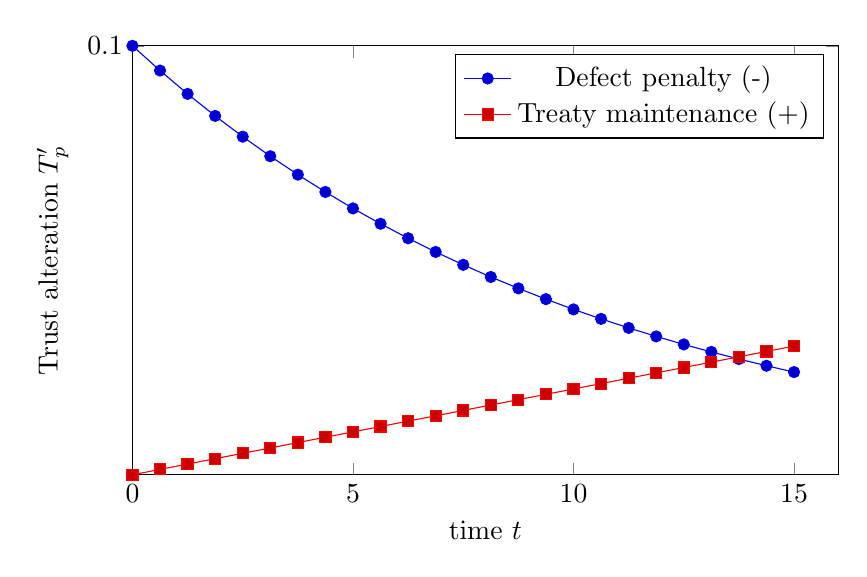
\begin{tikzpicture}
  \begin{axis}[ 
    width = 300,
    height = 200,
    xlabel= time $t$,
    ylabel={Trust alteration $T'_p$},
    xtick = {0,5,10,15},
    ytick = {0.1},
    xmin = 0,
    ymin = 0,
    xmax = 16,
    ymax = 0.1,
    domain = 0:15
  ] 
    \addplot {(1.1^(-x)/10};
    \addplot {0.002*x};
    \legend{Defect penalty (-), Treaty maintenance (+)};
  \end{axis}
\end{tikzpicture}
\caption{Treaty Trust-processing}
\label{fig:graph1}
\end{figure}

It is crucial to understand that the trust value assigned to different players in our system is not an indicator of how reliable they are. A player could for example reject a peace proposal and reliably not attack you consistently. But due to our expectations of the norms of peace, we expect no player nor bot to have this behavior. As such, in our system we choose to implement 'trust' as a fitness for choosing whom we should ally ourselves with, in addition to guiding how paranoid we should be against every other player. Having peace with someone you do not trust should be possible, but internally the bot should be paranoid in regards to defending his borders. The justification for such a possibility is for the untrusted player to have a chance to redeem itself if it chooses to adopt a more cooperative strategy. Given the decay of treaties, we can safely assume that the closer they are to diminishing, the more paranoid we should be. To repeat the initial statement of this section regarding seeing every player we do not have any treaty with as hostile, we assign them all with a full level of paranoia ($P = 1$). Every treaty initializes with an paranoia equal to the relevant powers current trust value. 

\subsection{Paranoia}
\
  \[ P_p = \left\{ 
  \begin{array}{l l}
    1 - \Big( D^{-t} \cdot T_p \Big) & \quad \text{for $T > 0$} \\
  1 & \quad \text{for $T = 0$}
    
  \end{array} \right.\]
\begin{figure}[H]
\centering
\begin{tikzpicture}
  \begin{axis}[ 
    width = 300,
    height = 200,
    xlabel= time $t$,
    ylabel={Paranoia $P_p$},
    xtick = {0,5,10,15},
    ytick = {1},
    xmin = 0,
    ymin = 0,
    xmax = 15,
    ymax = 1,
    domain = 0:15
  ] 
    \addplot {1-((1.1^(-x))*(0.8))};

  \end{axis}
\end{tikzpicture}
\caption{Paranoia processing. $T$ = 0.8}
\label{fig:graph2}
\end{figure}


Paranoia [0-1]  is a value attached to any power within an instance of a game which offers us the ability to predict whether or not we should expect them to defect. A procedure to reduce paranoia of any power we already have a treaty with is to re-iterate the initial proposal. In practice it is equivalent to ask our ally 'is our deal still on?'. To attend the issue regarding a deadlock of two fully righteous powers who never wishes to break a treaty, one will eventually ask if the deal is still on in which the other is at liberty to decline. As a result, this solution to breaking peace/alliance is possible without breaching any trust.


\subsection{Support obligations of alliances}

Within a conjoined alliance treaty together with power A, there lies an agreement to conduct both defensive and offensive support moves against power B. However, considering the fact that there can only be one winner of power B’s Supply Centers, the alliance can only be mutually beneficial if both parties divide the spoils of war. However, there might be possible moves towards gaining a Supply Center given the accessibility of one's own units if they were not requested somewhere else by our ally. If one would ignore how other players viewed us ($R$= 0), it would be rational to reject this request. This is not a fair deal for the other party as it can be exploited. A solution is needed which makes us sensitive to injustice in terms of our spoils and our ally's spoils.

 In addition we also want a model of appropriate conduct if we would want to be righteous, implying that we would be permissible if the other party declined supporting us if we knew we were in debt - that is, knowing he has currently been supporting us more than he has received from us. But even if our personality is unrighteous, we should also recognize those powers who are vulnerable to be exploited, namely altruists.

The function essentially captures the underlying obligation for allies to reciprocate support-moves. If a power asks for support all the time without reciprocating, its trust will decrement per support they REJECT when they owe us support. Although, whenever they  ACCEPT our request while we still owe them, we increment their trust on the basis of them being altruistic. Given the fact that trust-values are altered online, the support-favor $\sigma$ is stored as an attachment for every power per game. $\sigma > 0 $ implies you owe them supports, while $\sigma < 0$ implies they owe you. In addition, we have a variable for how intolerant we should be for deviation of reciprocity equilibria ($\sigma$ = 0), defined as $S$.\\


  \[ T'_p = T_p + \left\{ 
  \begin{array}{l l}
    (S \cdot \sigma_p)^2 & \quad \text{if $\sigma_p > 0$ \& ACCEPT}\\
    -(S \cdot \sigma_p)^2 & \quad \text{if $\sigma_p < 0$ \& REJECT}\\
    \text{0} & \quad \text{if ($\sigma_p \le 0$ \& ACCEPT) or ($\sigma_p \geq 0$ \& REJECT)}
    
  \end{array} \right.\]
  \\
\begin{figure}[H]
\centering
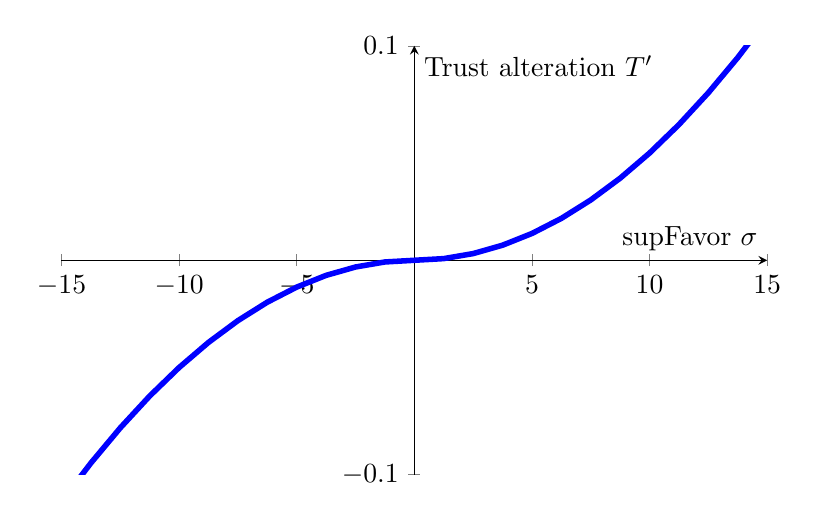
\begin{tikzpicture}
  \begin{axis}[ 
    width = 300,
    height = 200,
    axis x line = middle,
    axis y line = middle,
    xlabel= supFavor $\sigma$,
    ylabel={Trust alteration $T'$},
    xtick = {-15,-10,-5,0,5,10,15},
    ytick = {-0.1,0,0.1},
    xmin = -15,
    ymin = -0.1,
    xmax = 15,
    ymax = 0.1,
    domain = -15:15
  ] 
    \addplot [blue] [line width=2pt] {(x/abs(x))*((0.0005*x^2)};
  \end{axis}
\end{tikzpicture}
\caption{Support Favors. $S$ = 0.0005}
\label{fig:graph3}
\end{figure}

\subsection{Trust summary}

A consequence of the trust mechanics should leave exploiting players to be the least favorable alliance partners. This puts them at a severe disadvantage, as the remaining powers available for alliances most likely have a low trust value themselves. If two exploiting powers would team up, they would  both be forced to spend resources to defend against each other instead of opimizing an assault on their common enemy.

Cooperative players with a high righteousness will prefer each other as allies, without the disposition of a high paranoia. Their mutual trust boosts their utility.
\
As we have now covered the trust mechanics, the remaining personality factor is that of trust initialization for new players our bot meets. A value of 0 implies that its fully cautious at the start of treaties, whereas 1 implies full naivety of opponents exploitative capabilities. Below is a brief overview of events in the game which alters trust of other powers.\\
\
\\
\textbf{Incrementation:}
\begin{itemize}
\item {Every phase a treaty is maintained}
\item {Getting support from an ally you consider altruistic}
\end{itemize}
\textbf{Decrementation:}
\begin{itemize}
\item{Defect in upholding a treaty (backstab)}
\item{If you get a rejection in your support proposal from an ally which you deem exploitive.}
\end{itemize}
\section{Gain system}


In order for our AI to know where it should move it's units to, we make use of a gain system. For every province we calculate a gain value. This value signifies the importance of this province based on a variety of properties and heuristics. We weigh this gain with factors such as likeliness to succeed and whether we defect allies by moving to this province. 

\subsection{Gains}  

For each province the gain value signifies the importance of that province. To calculated the gain, we have selected a number of properties which we believe makes a province important (But can very easily be extended and adjusted). We divided these into four categories. 

\begin{itemize}
\item Supply gain
\item Defend gain
\item Counter gain
\item Kill gain
\end{itemize}

\subsubsection{Supply gain}
\label{sec:supplygain}
The supply gain is given to provinces which contain a Supply Center. In order to win the game one has to control more than half of all the Supply Centers. Also, the number of Supply Centers you control determines how much units you are allowed to have. Therefore, capturing Supply Centers is crucial to winning the game and these provinces are important and we give these a gain. There are however different types of Supply Centers we have to consider. 

Supply Centers can be controlled by a power. If a Supply Center is not controlled by us (so either neutral or under control by any other power), we can potentially take over this Supply Center. We give these a gain $g_{supply}$. Supply Centers we control have no real gain as we can not take them over again. However, in the case that there is nothing more important to do, we would prefer units to move to one of our Supply Centers as a means of defence. We therefore give a small symbolic gain $g_{ourSupply}$ to Supply Centers we own. 

Some Supply Centers are home Supply Centers. These are home to a specific power and a power can only build new units on his home Supply Centers. Additional to the importance of normal Supply Centers, capturing a home Supply Center from a power effectively disables this power from building new units there. Therefore we give these a different (higher) gain $g_{home}$. We only do this when this home Supply Center is under control by the corresponding power. If this is not the case, then this power is already blocked from building units there and there is no additional gain from taking this. In this case we treat is as a normal Supply Center and give gain $g_{supply}$.

Following this rule, our own home Supply Centers are also very important. As with normal Supply Centers, if we control them they get a small gain $g_{ourHome}$. However, if a home Supply Center is under control by another power it is very important to get it back in order to build new units. In this we assign a very high gain $g_{takenHome}$. 

\subsubsection{Defend gain}
\label{sec:defendgain}
Without defending the Supply Centers we already control, they will just as easy be taken back from us. The defend gain is therefore given to Supply Centers we control and are under threat. In order to do this we first have to quantify threat. We calculate the threat by a weighted sum of the first and second order enemies from the same power (e.g. the enemies one tile away and the enemies two tiles away respectively). 

$$threat = max_{threat}\{ threat : C_1 \sum_{i} e^{1}_{ij} + C_2 \sum_{i} e^{2}_{ij}\}$$

Where $e^1_{ij}$ and $e^2_{ij}$ are the ith respectively first and second order enemy units of power j. The treat is then the maximum threat of the threat each power. This assumes that the enemies will not cooporate, but the system can be easily adjusted to account for this as well (However, we would first need some assumptions on  alliances in the belief base). 

We have chosen to give the Supply Center a defend gain $g_{defend}$ if $threat > \varepsilon_{threat}$. As we belief that defending home Supply Centers is more important these get a different gain $g_{defendHome}$. 

\subsubsection{Counter gain}
\label{sec:countergain}
Using only the aforementioned gains, we perceived that units on threatened home Supply Centers displaying  ``camping'' behaviour. The unit keeps defending the home Supply Center from a neighbouring enemy whereas the neighbouring is interested in the home Supply Center and hence does not move away. We therefore introduced a high counter gain $g_{counter}$, to provinces adjacent to a home Supply Center and containing an enemy unit. This way, instead of endlessly holding the home Supply Center, units will start to make offensive moves against adjacent enemies driving the threat away instead of waiting for it to go.        

\subsubsection{Kill gain}
\label{sec:killgain}
Another thing we also witnessed by watching our AI play is that very often units of a power are on the far side of the map - far from any support. This units are often left unattended as a single unit is not considered a threat. We therefore introduced a kill gain $g_{kill}$. This is a very high gain for a province containing a lonely enemy unit (no other enemy units as close as two tiles away), and this unit has limited provinces $< \varepsilon_{kill}$ to retreat to - likely causing it to disband when attacked. 
Another issue solved by this, is that very often the last living unit of a power is left unattended and sometimes even regains considerable power. 

\subsection{Smoothing gains}
Provinces adjacent to provinces with a high gain are inherently important. This is because moving to that province brings us closer to the high gain province. Therefore it is important to apply some kind of smoothing to the gains, in order to reflect this importance of adjacent provinces. We have experimented with various smoothing methods and kernels and eventually settled with: 

$$g_{smoothed} = max(g_{base}, C_{s} max_{g}\{g : g^1_i\})$$

Basicly the smoothed gain is the maximum gain of all first order neighbours gains $g^1_i$, weighed with a constant $C_s$. In the case that the province already has a gain higher than this we will use the orignal base gain $g_{base}$. 

Due to smoothing the differences of gains between provinces decreases. In order to account for this we square all gains after the smoothing. 


\subsection{Support}

In order to prepare a movement, it is important to know whether the movement can be effective. Consider the situation where a province is occupied by one enemy unit, then it is useless to try to move to that province with only one unit. In this case at least two units are needed to kick the enemy out, and perheps additional units are needed to cope with enemy support. The gain system calculates the amount of units that is needed to invade a province. This is done by keeping track of all units that possibly can support each province, as well for the own power as for the enemy powers. At least one unit is needed when a province is not occupied by an enemy unit, and at least two units are needed for a occupied province. For each possibly supporting enemy unit, a unit from the own power has maybe to support. But it is not certain whether this unit needs to support, since it is not possible to know on forehand whether the enemy unit will support. To cope with this uncertainty, we incorparated a risk variable. This variable determines how large the support needs to be. It could become possible to move to an unoccupied province with only one unit and without any further support, while the enemy has two potentially supporting units. For each of the units that can support, a check is done whether a random value is larger than $\alpha_{sup}$ and the number of support is increased by one when this evaluates true. However this does not determine which units need to support, only how much units need to support in the case that this province is going to be invaded. We have chosen to defined $\alpha_{sup} = risk^{k}$ where risk is between 0 and 1, and k is the amount of enemy support and $k>0$. By the amount of enemy support is meant the highest enemy support of all individual enemies. We choose for an exponential function since we believe that when something is important and hard, it is better to strike hard. Besides a human experiences a move whith too less units as a stupid move. 

\subsubsection{Drawback support}
Consider the case that all units already have a task assigned, except for one unit. This unit could move to an unoccupied province surrounded by three enemy units. Since the enemy support is quite high, it is likely that there also will be a high number support assigned to this province. As result this province is filtered out as untakeable. But how realistic is this? Since it concerns the last unit, the priority of the province won't be very high and therefore it is not likely that the enemy would use so much units on this province. To cope with this drawback, the risk variable should be slightly increased every time a target is chosen. In this way very low risks are taken with high priority targets, and more risk is taken with lower priority targets. 

\subsection{Weighting}
So far the importance of an province is only expressed by it\'s gain. But the importance must also include other factors such as the likeliness to succeed and whether allies are defected. Therefore a weight value is determined for each province which depends on the following factors:

\begin{itemize}
\item Gain
\item Likeliness to succeed
\item Shared units
\item Probability to defend
\item Probability to attack
\end{itemize}

The weight is initialized at the gain of the province. It is important to only invade a province when it is very likely to succeed. The amount of support needed includes already a risk factor, as exlained before. Therefore it is not necessary to do another considerations about succes at the weights, it is only important whether the province is takeable or not. So the weight is set to zero when the support of our power is lower than the estimated resistance of the enemy.

At each movement most of the units have mulitply options to move to, so on a first thought is would be logical to give a penalty for provinces that need a lot of units that also can be deployed somewhere else. However this doesn\'t stroke with our tactic of chosing a few main objectives and succeed on these. Consider the case where a very important home Supply Center is under attack and needs to be defended by a lot of units. However all these units are able to take over another Supply Center without any resistance, which has a high gain. Therefore the defence of the home Supply Center gets a huge penalty for it\'s shared units, and would maybe not be the top priority objective. But it would be stupid to take over all the free Supply Centers while the home Supply Center is lost, which implies that the annexation of the free Supply Centers is for nothing since no new units can be build. Therefore we decided to set the penalty to zero. 

In Diplomacy plays collaboration a key role, one can hugly benefit from a peace treaty since it has not to spend it\'s units on defence. The weight of a province can be lowered when it is defended against a power that is trusted. Therefor we multiply each defensive gain with $\alpha_{defend}$, which lowers the weight. The defensive gains are the defend gain and the counter attack gain. At this point we decided that $\alpha_{defend}$ is a binary value, either 0 or 1. This is done since $\alpha_{defend}$ is also used in the determination of support needed, and there does not exist such thing as supporting with one third of a unit. 

The last factor that influences the weight is the probability that our power is willing to attack a friendly power, namely the $R$ value described in the trust section. Sometimes the gains of a province are so high that it can be beneficial to attack it regardless the fact that it is owned by a friendly power. This consideration is realized by using an $\alpha_{attack}$ factor. This factor is 1 for all powers for which no peace treaty is declared. For each friendly power this factor has a value between 0 and 1, where a value of 0 means that our power will not attack that power. $\alpha_{attack}$ is multiplied with all offensive gains, the Supply Center gain and the kill gain. It is not wise to attack a province with a very low weight that is owned by a friendly power, since it is not benificial to defect a friendly power for so less gain. Therefore the weight of a province owned by a friendly power needs to be higher than $\varepsilon_{attack}$, and when this is not the case the weight is set to 0. 

\subsection{Movement Phase} 

During the movement phase the units get orders assigned to defend or invade provinces, or to support another units. The gains system is used to determine which provinces need to be taken by which units. A prioritized list of provinces is fetched from the gain system, where the first province in the list represents the most important objective. This list also contains all the provinces which are not takeable, so these are first filtered out. Next one of the provinces is chosen to invade, or to defend in the case that there already was a unit of our power on it. The units needed for this attack can also be fetched from the gain system, together with the information how they can move to this province. From this the orders are constructed and the gain system is updated. Some units are used, so these will not be available for another attack this phase. Units are used by either moving to an province or by holding on a province. So these provinces will not be available to move to this phase. During the update of the gain system the used units and provinces are removed from it, and for each province is reconsidered whether it is still takeable with the remaining units. After the update a new prioritized list can be fetched to determine the next objective. 

The objective to pick could be just the first one in the prioritized list, since this is the most important one. But this has the risk of getting stuck in a local maximum, sometimes an objective with a lower priority can yield a larger result later on. So it must also be possible to pick an objective with a lower priority. Each province $P_{i}$, or objective, has a weight $w_{i}$ that represents it\'s priority. All weights are summed up to compute the total weight $W=\sum_{i}w_{i}$. A random number $r$ in the interval $[0...W)$ is computed to determine which objective will be picked. The first objective $P_{0}$ will be picked when $r$ lies in the interval $[0...w_{0})$ and a province $P_{i}:i>0$ will be picked when $r$ lies in the interval $[w_{i-1}...w_{i}]$. The probability of chosing an objective is proportional to it\'s weight. But this has a disadvantage. Consider the case where one objective has a very height weight, and a lot of objectives have a quite low weight. The sum of all the lower weights can be higher then that one very high weight. In this case the probability of picking an objective with a low weight is larger than the probability of picking the most important one. This does not correspond with the idea of picking the most important objectives. Therefore we discard all objectives that do not have a weight higher than half of the weight of the most important objective, thus an objective is discarded when $w_{i} < \frac{w_{0}}{2}$.

\subsection{Retreat and Build Phase}

During the retreat phase, units that are defeated must retreat from their current province. We have to order to which adjacent province they have to retreat. We simply do this by sorting the available option by gain and retreat the unit to the option with the highest gain. If there is no option we have to disband the unit. 

During the build phase the number of units you have should be equalized to the number of Supply Centers you control. Hence, if you lost Supply Centers you have to remove units and if you gained Supply Centers you can build units (But only on your home Supply Centers). In the case we have to remove units we will delete the units which are on the provinces with the lowest gains, as these units are probably less of use in the next turn. In the case we can build units, we will build units on home provinces with the highest gain. This indirectly implies that we we build units on the most threatened home Supply Center, as those gains will be the highest. If there all our home Supply Centers are occupied, we have to waive that build.    

\subsection{Gain values}

In \autoref{table:gains} we present the values selected for the various gain variables introduced in the previous sections. 

\begin{figure}[H]
\centering
\begin{tabular}{| l | c |}
  \hline            
  {\bf Gain} & {\bf Value}\\
  {Supply Gains} &  \\
  $g_{supply}$ & 3.0 \\
  $g_{ourSupply}$ & 0.25 \\
  $g_{home}$ & 3.2 \\
  $g_{ourHome}$ & 0.3 \\
  $g_{takenHome}$ & 5.0 \\
  {Defend gains} &  \\
  $g_{defend}$ &  3.0 \\
  $g_{defendHome}$ & 3.2 \\
  {Counter gain} & \\
  $g_{counter}$ & 5.5 \\
  {Kill gain} & \\
  $g_{kill}$ & 5.0 \\
  \hline  
\end{tabular}
\caption{Values choses for the various gain variables}
\label{table:gains}
\end{figure}

We started with simple choosing some value for $g_{supply}$. Following \autoref{sec:supplygain} we chose a slighty higher value for $g_{home}$, much low values for $g_{ourSupply}$ and $g_{ourHome}$ and a much higher value for $g_{takenHome}$. The rest of the values were set and all values were tweaked by trial and error (e.g. watching the bot play and try to reduce dumb moves to a gain). Automatic learning on these values might be possible but would be very hard, as it is difficult to determine whether a change is succesful or not. Also these gains might differ a lot for playing a diffent power and depend on alliances and such. Instead we believe that implementing more heuristics is the key. 

\section{Implementation}
For our implementation we used DAIDE, the Diplomacy AI Development Environment:
\begin{sloppypar}
\noindent\url{https://sites.google.com/site/diplomacyai/home/daide}
\end{sloppypar}
It provides an environment where new AI’s can be created and compete against each other. DAIDE provides the syntax of all the communication with the server, the communication protocols and the server itself. This way we only have to focus on the AI itself. 
There are several AI’s available for DAIDE to compete against, as well as a  so called AImapper to visualize the action. Communication with the server is done through simple TCP/IP connections, this way it is possible to create a bot using any language, as long as you can handle TCP/IP. 
For our own specific implementation we build upon the ‘Diplominator’, which is a very simple AI that we stripped of almost everything except the communication functions. There are other frameworks available that also provides functions to parse the DAIDE syntax but since we wanted more control and a way to learn the syntax we created our own parsers. As for programming language we settled for Java, mostly because we needed a cross-platform language because some of our group use Linux. 

\subsection{User manual}

\subsubsection{AIServer}
In order to run our AI, you first need an AIServer which runs the game and to which the AI can connect. In order for our AI to fully function we use the AIServer that can be downloaded from: 

\begin{sloppypar}
\noindent\url{http://johnnewbury.me.uk/diplomacy/downloads/aiserver/aiserver-0.38~1.1-release-notice.htm}
\end{sloppypar}

The AIServer contains a Windows executable file but also runs perfectly under Wine on Linux. Upon running this executable the user is presented with various options. For our AI, make sure that the \textit{Log All Messages} option is on and the press level is set to a minimum of 20 (otherwise the server does not allow for alliance negotiation). A new game can now be started by clicking the \textit{New Game} button. This opens up a lobby, and the game will start as soon as 7 players have joined.     

\subsubsection{DodoAI}
In order to compile and run the Java code you can either import it an Java IDE such as Eclipse or use the command line. For the latter option we have included a makefile in the $src$ directory. Make sure a Java SDK (OpenJDK or Sun) is installed. After a succesfull compilation (ignore the warnings) you can run the program by running the DodoAI class with Java. Assuming a Unix-like operating system:       
\begin{lstlisting}[frame=single] 
cd location/of/repository/src/
make
java ai.dodo.DodoAI [ip] [port] [options]
\end{lstlisting}

Where \textit{ip} should be the ip address of the server - if run locally on the same machine use \textit{localhost} for this. \textit{port} is the port on which the server is listening. The default option for this is 16713 but can be adjusted in the AIServer settings. After these two arguments, several options can be set with flags

\begin{description}
\item[-n [name]] Using the -n flag the name for the AI (default DodoAI) can be changed. 
\item[-l [filename]] Using the -l flag, you can set the location of the server log file. Using this log file the AI will extract the names of all AI's and corresponding power from the server log file. Though this is not allowed by official Daide rules, this allows our AI to know who plays which power during the game. This is necessary as one of our goals was to include reputation in our AI. Note that this option is only possible if the server runs on the same machine or has remote access to the server log file.  
\item[-f [filename]] The -f flag can be used to set a personality file for this AI in order to create a unique personality. An example of a personality file can be found somewhere TODO. Note that the personality file includes a name which will override a name given a name with the -n flag.  %TODO!!%.  
\item[-k] If the -k flag is given, the AI will require a keypress in order to submit its orders at the end of a turn. This is very useful when observing an AI-only game, the game is over so fast that is impossible to see what happened. We recommend running a single instance of DodoAI with the -k flag (Instead of all 7), as the rest of the AI's will automatically have to wait for this instance.  
\end{description} 

\subsubsection{AIMapper}
In order to visualize the game or play against our AI yourself, you need the AIMapper. This AIMapper can be downloaded from: 

\begin{sloppypar}
\noindent\url{http://johnnewbury.me.uk/diplomacy/downloads/aimapper/aimapper-0.41~1.1-release-notice.htm}
\end{sloppypar}

As with the AIServer the AIMapper comes as a windows executable, but is fully functional under Wine in Linux. You can join as either an observer (only watch the game) or player (play yourself). 

\section{Conclusion}
For this project we have created an AI, DodoAI, that can play the game Diplomacy on its own. Our initial goals was to have an AI that can handle level 20 press, distinguish allies and foes with an extensive trust system and dynamically give orders based on weights and gains. Unfortunately we were not able to complete all of those goals. We now explain why we were not able to complete those goals, starting with press. 
 
From all of the online bots that are created for Diplomacy, almost none of the existing bots can handle press above level 10. Seeing opportunity in this fact, one of our goals was to implement an AI that would go beyond most of the existing AIs by being able to handle those higher press levels. But there is a reason that so little bots can handle higher press, negotiations can become very complicated very fast. Albert, universally seen as the best Diplomacy-playing AI available, has been four to five years in development and is the only available AI that can handle level 20 press. It is no big surprise that we were not able to accomplish the same feat in the limited time available.  
 
One of the most important reasons that counts for all unfinished functions is the scope of the problem. Each extra form of negotiation means another set of possibilities to take into account. Alliance and Peace are fairly simple but uninteresting on their own. Adding anything atop of that increases the complexity exponentially. For example: at the base are the orders generated from the weights and gain system, but if you have allies you need to adjust the gain for the allied provinces. The AI may attack an ally when above a certain paranoia threshold, but maybe you need that ally to defend your eastern border. You also have peace with the power at your western border, the trust is low so you need to keep units there, but he just proposed an alliance, accept or reject? And what are the consequences for your current set of orders while several of your allies propose a multitude of order proposals, which one do you pick? Or maybe it is better to keep your original set of orders, but you are in an alliance with them so rejecting them might be bad later when you are in trouble etc. The problems that arise from this example are mainly based on uncertainty, it is hard to determine what the best course of action is in any of the given situations, especially for an AI. Furthermore there is the technical problem of handling several proposals at once or the simultaneous sending and receiving of similar proposals. It is possible to always agree but because of our trust system it is hard to agree upon things the bot knows it cannot keep. It became clear that for some of our goals it might not be possible to implement them the way we wanted too. The two specific order proposals that come with level 20 press are listed below, with an extra explanation of why it proved too difficult. 
 
XDO or Order Proposal. The XDO proposal allows the suggestion of order proposals for the units of other powers.  This is probably the most useful arrangement at this level or below, it actually allows your allies to act like allies. Without XDO there is hardly any difference between peace and alliance, in both you agree not to attack each other, in the latter you agree to attack another power. But it is never specified how or when, and due to the nature of giving orders you can never support an ally in their attacks if you do not know where they are moving to. It is also a huge factor to consider for betrayals, does an ally actually acts upon your proposed orders or does he betray you when you are counting on them? This leads to many more possibilities and thus complexity, especially since you can propose any legitimate order. 
We agreed fairly soon that we would only focus on proposing support orders to either hold or attack a province. The other forms of orders like convoy, move or hold are unnecessary to handle in regard to alliances, you only want them to support you so you can take or defend a province. So far we have implemented a large portion of the framework to handle order proposals, but it still lacks proper functions that can initiate an order proposal or determine when to accept incoming proposals. Deciding these two things proved simply too difficult to do.  
 
DMZ or Demilitarized Zone. The DMZ proposal sets a province as demilitarized zone, agreeing that none of the powers involved will move their units there. Breaking this pact would immediately cause a war and break any other arrangements the powers have. It is a very useful arrangement, agreeing that a certain province is off-limits severely lightens the need to guard certain areas. It also acts as a failsafe for betrayals. The betrayer first needs to go through the DMZ before being able to do any damage. 
 
The trust system is implemented and working, it keeps track of all the other powers and alliances and determines the level of trust dynamically and accurately. This is something that the existing AI’s do not have and could prove very valuable in defeating them. Logically, the DodoAI’s that trust each other should stick together while avoiding the dishonest ones. 

Something that other bots don’t have is our weights and gains system, which even works above expectation. Where other bots need to process every possible move, we can dynamically adapt to any new situation, making processing time very low. Also the addition of new parameters like trust and paranoia are easy to implement, leading to much more complex behaviour. Peace and alliance is taken into account by simply adjusting the weight of peaceful provinces. The system can be further optimized by tweaking a few values or adding some heuristics, instead of going through hundreds of combinations of moves like other bots. This makes DodoAI much more dynamic and potentially very powerful. It can already easily win against the Diplominator, with an optimization using neural networking it might defeat Albert one day. 



% \begin{thebibliography}{1}

%   \bibitem{notes} Pacheco, J.M., Santos, F.C., Souza, M.O. and Skyrms, B., {\em Evolutionary dynamics of collective action in N-person stag hunt dilemmas}  2009.

%   \bibitem{impj}  da Costa Ferreira, A.F., {\em DipBlue: a Diplomacy Agent with Strategic and Trust Reasoning} For Jury Evaluation.

% \end{thebibliography}

\bibliography{references}{}

\end{document}